\subsubsubsection*{EfficientPS}
\label{sec:EfficientPS}

EfficientPS é uma solução eficiente para a segmentação panóptica, proposta no artigo \citeonline{mohan2020efficientps}. Em seu repositório na internet \citeonline{efficientpsGit}, há algumas recomendações de tecnologias utilizadas para desenvolver e testar o modelo. Embora possa funcionar em outros cenários, não há suporte dos criadores para tais aplicações. Essas tecnologias são: uma distribuição de sistema operacional\footnote{Programa que gerencia a parte física de um computador; meio termo entre o usuário e a parte física do computador.} com núcleo Linux, conforme descrito em \citeonline{redhat2023}; a linguagem de programação Python na versão 3.7, que, segundo \citeonline{analyticsindiamag2023}, é amplamente utilizada no campo da IA devido à sua simplicidade e às diversas bibliotecas que facilitam a criação de modelos complexos; o PyTorch na versão 1.7, que, de acordo com \citeonline{pytorch2023}, é uma estrutura baseada na biblioteca Torch, visando facilitar a criação de modelos de aprendizado profundo; o CUDA Toolkit na versão 10.2, que, segundo \citeonline{cudatoolkit2023}, é uma biblioteca para proporcionar aceleração do processamento com placas de vídeo da marca Nvidia; e, por fim, o GCC nas versões 7 ou 8, que, conforme \citeonline{gcc2023}, é um compilador das linguagens C e C++, frequentemente utilizados em bibliotecas Python, como o PyTorch, por exemplo.

\subsubsubsection*{Arquitetura}

O artigo apresenta uma arquitetura que se inicia com um \textit{backbone} — parte responsável por identificar características —, utilizando uma Rede de Pirâmide de Características (RPC)\footnote{Estrutura de pirâmide para extrair características em várias escalas de uma imagem \space\cite{piramide}} de dois caminhos, seguida de dois cabeçotes paralelos: um para uma arquitetura de segmentação semântica, de autoria própria, e outro de instância, com modificações baseadas na topologia Mask R-CNN. Finalmente, a saída dos dois cabeçotes é combinada no módulo de fusão panóptica para gerar a saída final com a imagem de segmentação panóptica. Esta arquitetura é ilustrada na \cref{fig:arqEP}.

\begin{figure}[ht]
	\caption{Arquitetura geral do EfficientPS}
	\centering % para centralizarmos a figura
	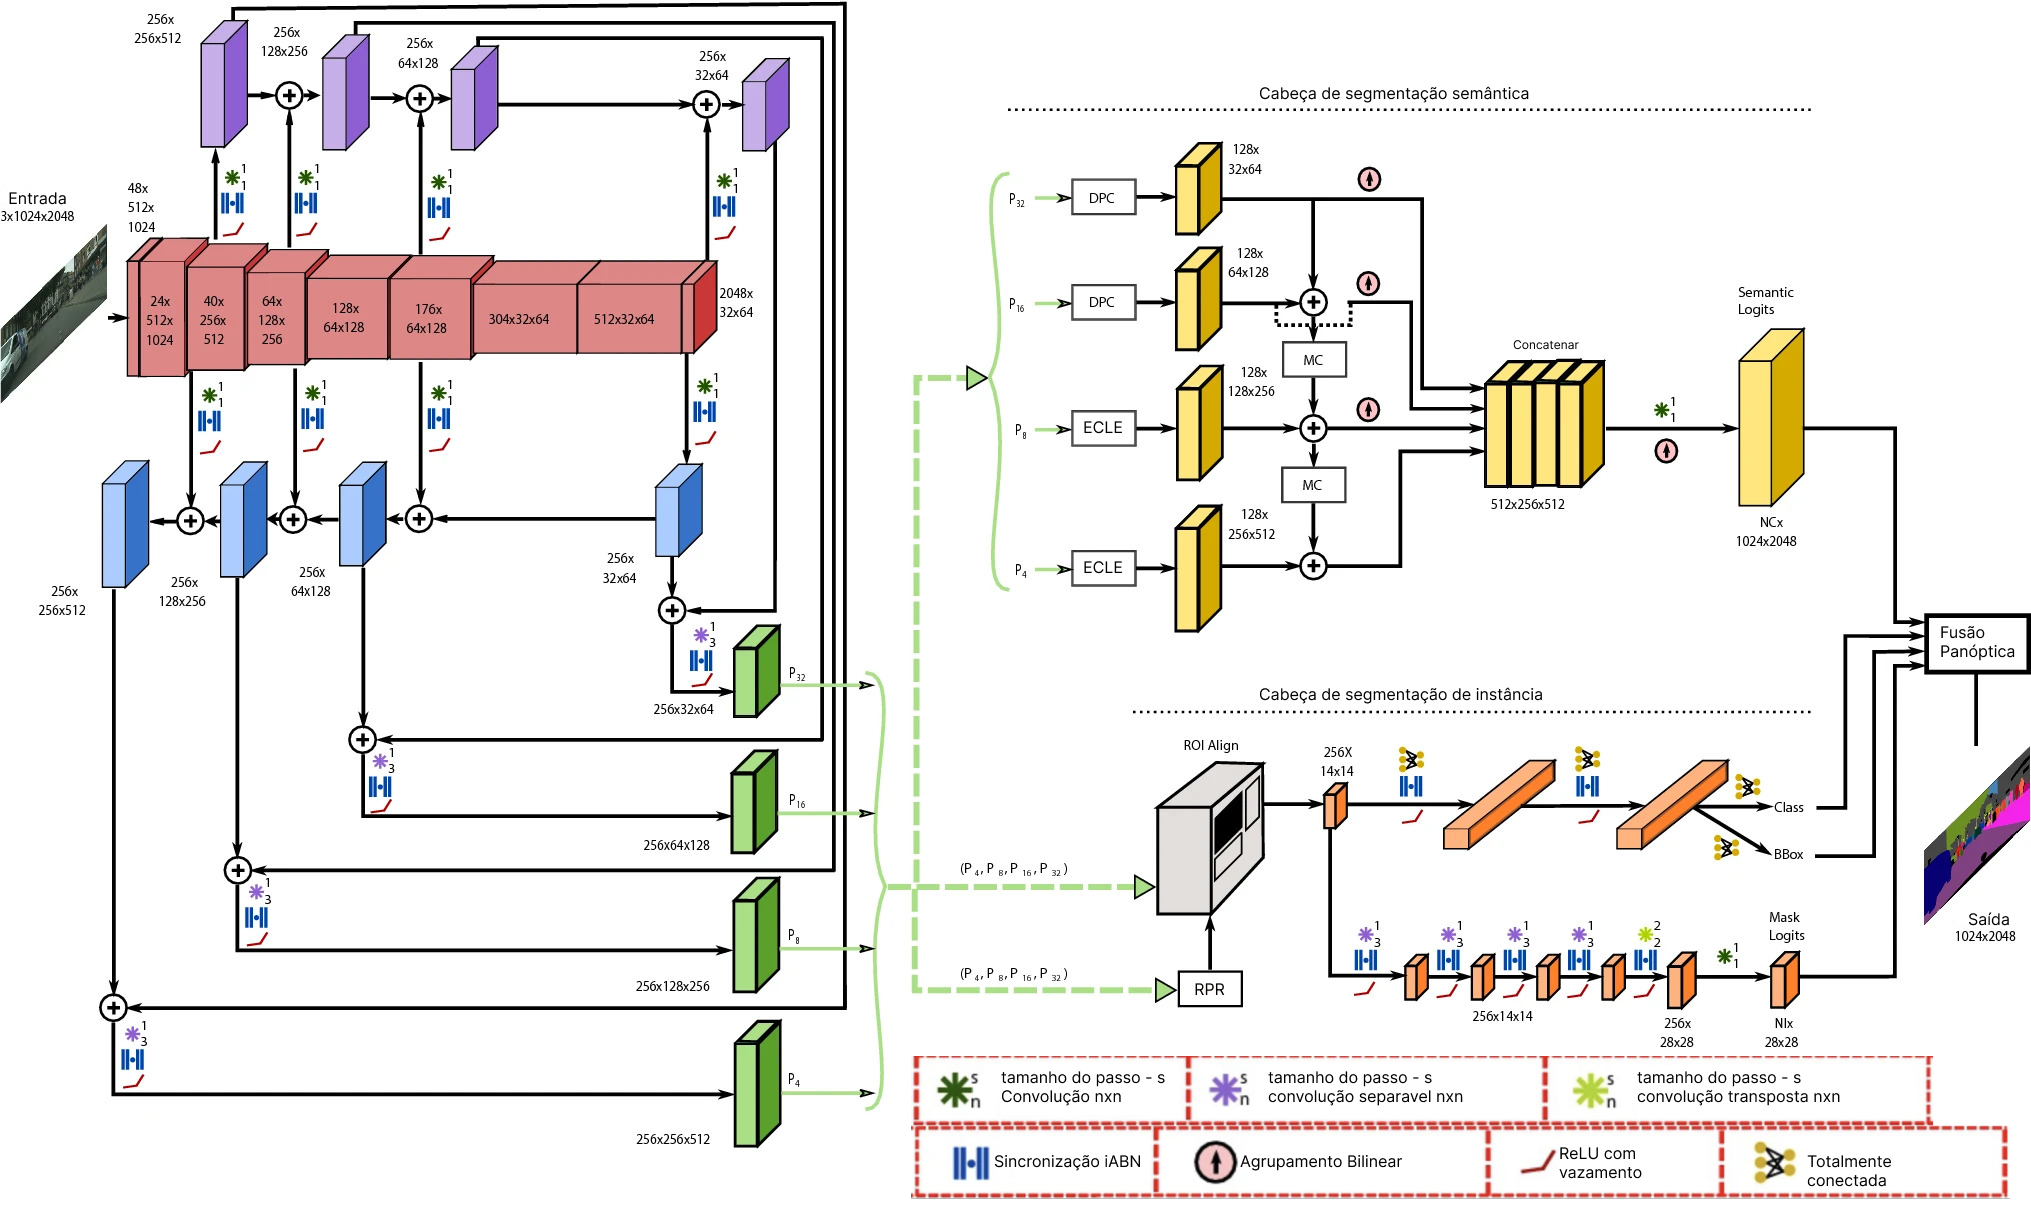
\includegraphics[width=15cm]{figures/arqEP.png} % leia abaixo
	\legend{Fonte: \citeonline{mohan2020efficientps}}
	\label{fig:arqEP}
\end{figure}

\subsubsubsection*{Backbone da rede}

A espinha dorsal — ou backbone — consiste em uma codificação combinada a uma bifurcação paralela usando RPC. O codificador é essencial para arquiteturas de segmentação e, para melhorar a capacidade de representação, é necessário aumentar o número de parâmetros e a complexidade. No entanto, neste artigo, os autores apresentam uma solução equilibrada neste aspecto. O codificador contém nove blocos (em vermelho), mostrados na \cref{fig:arqEP}, e as saídas 2º, 3º, 5º e 9º — da esquerda para a direita — correspondem aos fatores de redução de amostragem x4, x8, x16 e x32, respectivamente. Essas saídas se conectam à bifurcação paralela, que possui sentidos opostos, para gerar mais detecções de características. Posteriormente, é realizada uma combinação entre camadas de mesma dimensão, utilizando camadas de convolução separável em profundidade — que divide em etapas espaciais e de canal, aplicadas a cada canal e a cada pixel de saída, respectivamente —, resultando nas saídas \( P_4 + P_8 + P_{16} + P_{32} \) \cite{mohan2020efficientps, redes-neurais-convolucionais-separaveis-em-profundidade}.

\subsubsubsection*{Cabeçote de Segmentação Semântica}

O cabeçote de segmentação semântica, uma criação dos autores, é dividido em três módulos: o Extrator de Características em Larga Escala (ECLE) — ou Large Scale Feature Extractor (LSFE) —, destinado a capturar recursos finos em larga escala de forma eficiente; o módulo DPC, que deve ser capaz de capturar contexto de longo alcance, mas em pequena escala; e o módulo MC, responsável por mitigar a incompatibilidade entre recursos de grande e pequena escala nas camadas de agregação \cite{mohan2020efficientps}.

As quatro entradas do cabeçote, \( P_4 + P_8 + P_{16} + P_{32} \), são processadas separadamente. As entradas \( P_{16} + P_{32} \) — de pequena escala — alimentam dois módulos DPC paralelos, enquanto \( P_4 + P_8 \) — de larga escala — alimentam dois módulos ECLE paralelos \cite{mohan2020efficientps}.


\subsubsubsection*{Cabeçote de segmentação de instância}

Este cabeçote é derivado da arquitetura Mask R-CNN, e as modificações realizadas foram três: a substituição da convolução padrão por convolução separável em profundidade — para reduzir o número de parâmetros consumidos pela rede —, a substituição da camada de normalização em lote por iABN Sync\footnote{Normalização em lotes entre cores de GPU para aumentar o desempenho.} e a troca da função ReLU, definida em \cref{eq:relu_func}, pela função Leaky ReLU, definida em \cref{eq:relu_leaky_func} \cite{mohan2020efficientps, redes-neurais-convolucionais-separaveis-em-profundidade, serp-ai}.

\subsubsubsection*{Módulo de fusão panóptica}

O módulo de fusão panóptica é essencial para construir a imagem com segmentação panóptica. Nesta etapa, os resultados dos dois cabeçotes anteriormente explicados são combinados. Esta tarefa não é simples, pois requer uma lógica sofisticada para lidar com as sobreposições encontradas. O módulo foi projetado para ser adaptativo e usar as duas entradas de forma equivalente \cite{mohan2020efficientps}.

Resumidamente, o módulo aplica técnicas para reduzir o número de instâncias baseando-se na métrica logística — um valor numérico que pontua a confiança. Ele realiza agregações entre os resultados dos dois cabeçotes e desenha com fundo preto as instâncias de maior confiança. Posteriormente, preenche com a parte de \textit{stuff} — classes semânticas de menor importância — da entrada semântica \cite{mohan2020efficientps}.
